\documentclass[aspectratio=169]{beamer} 
\usetheme{Boadilla}
%typical packages
\usepackage{tikz,amsfonts,amsmath,pgfplots, stmaryrd}
\setcounter{MaxMatrixCols}{20}
\usepackage{subfig}
\usepackage{bookmark}
% Include the algorithm packages
\usepackage{algorithm,algorithmic}
\usepackage{ifthen}
\usepackage{minted}
\usepackage{verbatim}
\usepackage{subcaption}
\usepackage{multirow}  % For the multirow functionality
\usepackage{lmodern}   % Optional, for improved font rendering


\usepackage{graphicx}
\newcommand{\cK}{\mathcal{K}}

% Define the theorem environment
\newtheorem{theo}{Theorem}

\newenvironment{ftheo}[1][]
  {\begin{mdframed}\begin{theo}\ifthenelse{\equal{#1}{}}{}{\ (#1)}}
  {\end{theo}\end{mdframed}}

\usetikzlibrary{shapes,arrows,positioning}
\newcommand{\RR}{\mathbb{R}}
\newcommand{\norm}[2]{\left \lVert #1 \right \rVert_{#2}}
\newcommand{\abs}[1]{\left| #1 \right|}
\newcommand{\grad}{\nabla}

\newcommand{\eps}{\epsilon}
\newcommand{\Div}{\nabla\cdot}
\newcommand{\bn}{\mathbf{n}}
\newcommand{\bq}{\mathbf{q}}
\newcommand{\bm}{\mathbf{m}}


\newcommand{\bX}{\mathbf{X}}

\newcommand{\cT}{\mathcal{T}}
\newcommand{\cX}{\mathcal{X}}
\newcommand{\cY}{\mathcal{Y}}

\newcommand{\CG}{\text{CG}}
\newcommand{\DG}{\text{DG}}

\newcommand{\hmax}{h_{\max}}
\newcommand{\hmin}{h_{\min}}

\newcommand{\oneh}{\mathbb{1}_h}

\newtheorem{defn}{Definition}
% Define your custom colors
\definecolor{zzttqq}{rgb}{0.6,0.2,0}
\definecolor{ccqqqq}{rgb}{0.8,0,0}
\definecolor{zzqqqq}{rgb}{0.6,0,0}
\definecolor{qqqqff}{rgb}{0,0,1}

\usepackage{listings}
\usepackage{xcolor}
\definecolor{darkgreen}{RGB}{0,150,0} % A shade of dark green



\lstset{ 
  backgroundcolor=\color{white},   % set background color
  basicstyle=\ttfamily\small,      % basic font style
  keywordstyle=\color{blue},       % keyword style
  commentstyle=\color{darkgreen},      % comment style
  stringstyle=\color{red},         % string style
  numbers=left,                    % display line numbers
  numberstyle=\tiny\color{gray},   % line number style
  stepnumber=1,                    % the step between two line numbers
  numbersep=5pt,                   % how far the line-numbers are from the code
  frame=single,                    % adds a frame around the code
  tabsize=2,                       % sets default tabsize
  breaklines=true,                 % sets automatic line breaking
  breakatwhitespace=true           % breaks lines at whitespace
}
\captionsetup{justification=centering}
%\usepackage{showframe}


%\fvset{fontsize=\small, numbers=left} 

\newcommand{\mfile}[1]{
\begin{quote}
\VerbatimInput[frame=single,framesep=3mm,label=\fbox{\normalsize \textsl{\,#1\,}},fontfamily=courier,fontsize=\scriptsize]{#1}
\end{quote}
}

\newcommand{\Matlab}{\textsc{Matlab}\xspace}
\newcommand{\Octave}{\textsc{Octave}\xspace}
\newcommand{\Python}{\textsc{Python}\xspace}
\newcommand{\ipython}{\textsc{ipython}\xspace}
\newcommand{\numpy}{\textsc{numpy}\xspace}
\newcommand{\scipy}{\textsc{scipy}\xspace}
\newcommand{\matplotlib}{\textsc{matplotlib}\xspace}
\renewcommand{\thesubfigure}{\arabic{subfigure}}

\usepackage{pgf,tikz}
\usetikzlibrary{arrows}


\usepackage{listings}
\usepackage{xcolor}

\definecolor{codegreen}{rgb}{0,0.6,0}
\definecolor{codegray}{rgb}{0.5,0.5,0.5}
\definecolor{codepurple}{rgb}{0.58,0,0.82}
\definecolor{backcolour}{rgb}{0.95,0.95,0.92}

\lstdefinestyle{mystyle}{
    backgroundcolor=\color{backcolour},   
    commentstyle=\color{codepurple},
    keywordstyle=\color{magenta},
    numberstyle=\tiny\color{codegray},
    stringstyle=\color{codepurple},
    basicstyle=\ttfamily\footnotesize,
    breakatwhitespace=false,         
    breaklines=true,                 
    captionpos=b,                    
    keepspaces=true,                 
    numbers=left,                    
    numbersep=5pt,                  
    showspaces=false,                
    showstringspaces=false,
    showtabs=false,                  
    tabsize=2
}

\captionsetup{
  font=small,          % Select font size
  labelfont=bf,        % Select appearance of label
  margin=3em,          % Margin, left and right
  tableposition=top    % Formatting for captions above tables
}





\usepackage{mdframed}


\addtobeamertemplate{navigation symbols}{}{%
    \usebeamerfont{footline}%
    \usebeamercolor[fg]{footline}%
    \hspace{1em}%
    \insertframenumber/\inserttotalframenumber
}
\newcommand{\myfigure}[3]{
    \begin{figure}
        \centering
        \includegraphics[width=#1\textwidth]{#2}
        \caption{#3}
    \end{figure}
}
%typical tikz stuff
\tikzstyle{vertex}=[circle, draw, inner sep=0pt, minimum size=6pt,fill=white]
\newcommand{\vertex}{\node[vertex]}
\usepackage{pgf}
\usetikzlibrary{arrows}
\pagestyle{empty}
\definecolor{zzttqq}{rgb}{0.6,0.2,0}
\definecolor{uququq}{rgb}{0.25,0.25,0.25}
\definecolor{xdxdff}{rgb}{0.49,0.49,1}
\definecolor{qqqqff}{rgb}{0,0,1}


% --- PACKAGES ---
\usepackage{graphicx} % Required for including the logo

% --- PRESENTATION INFORMATION ---
\title{Adaptive Mesh Refinement for Obstacle Problems}

% The \author command handles both authors and their affiliations.
% \underline{...} highlights your name as the speaker.
% \inst{...} creates the superscript numbers for affiliations.
% \thanks{...} creates the footnote for your Master's university.
\author{\underline{Stefano Fochesatto}\inst{1} \and Ed Bueler\inst{2}}

% The \institute command lists the institutions corresponding to the \inst numbers.
\institute{
  \inst{1} Dept. of Computer Science, University of Colorado Boulder \\
  \inst{2} Dept. of Mathematics \& Statistics, University of Alaska Fairbanks
}

% The \date command is a great place for conference and event details.
\date{SIAM TXLA \\ September 28, 2025}


\begin{document}

 \begin{frame}
\titlepage
\end{frame}


\beamertemplatenavigationsymbolsempty

\begin{frame}{Overview}
	\tableofcontents
\end{frame}




%\section{Finite Element Methods for PDEs}
%\tableofcontents[currentsection]
%
%\begin{frame}
%	\frametitle{A Reference PDE Problem}
%	\begin{itemize}
%		\item Poisson Dirichlet Problem:
%		\begin{equation*} 
%			 \qquad  -\nabla^2u = f \text{ on } \Omega,  \qquad u =g_D \text{ on } \partial\Omega
%		\end{equation*}
%	
%		\item Example:
%		\begin{equation*}
%			\Omega = [-1, 1]^2
%		\end{equation*}
%		\begin{equation*}
%			u(x, y) = \dfrac{2(1 + y)}{(3 + x)^2 + (1 + y)^2}.
%		\end{equation*}
%		We find $-\nabla^2u = 0$ exactly, so $f = 0$ and $g_D = u|_{\partial\Omega}$.
%	\end{itemize}
%	
%	
%	\begin{figure}[H]
%		\begin{center}
%			\includegraphics[width=.50\textwidth]{Figures/ReferenceSolution.png}
%			\label{fig:Reference Problem 3D}
%		\end{center}
%	\end{figure}	  
%\end{frame}
%
%
%
%\begin{frame}
%	\frametitle{Weak Form for Poisson Dirichlet Problem}
%		\begin{definition}[Weak Form]
%			 Find $u \in H^1_{g_D}(\Omega)$ such that,
%			\begin{equation*}
%				\int_{\Omega} \nabla u \cdot \nabla v = \int_{\Omega} vf \text{ for all } v \in {H}_{0}^1(\Omega)
%			\end{equation*}
%			Where the solution and test subspaces are, 
%			\begin{equation*} 
%				H^1_{g_D}(\Omega) := \{u \in {H}^1(\Omega): u = g_D \text{ on } \partial \Omega_D\},  
%			\end{equation*}
%			\begin{equation*} 
%				{H}_{0}^1(\Omega) := \{v \in {H}^1(\Omega):  v = 0 \text{ on } \partial \Omega_D\}.
%			\end{equation*}
%
%			\begin{equation*} 
%				{H}^1(\Omega) := \{u: \Omega \to \mathbb{R}: u, \frac{\partial u}{\partial x}, \frac{\partial u}{\partial y} \in L_2(\Omega)\}. 
%			  \end{equation*}
%	\end{definition}
%\end{frame}			
%
%\begin{frame}
%	\frametitle{Finite Dimensional Weak Form for Poisson Dirichlet Problem}
%
%	\begin{columns}[c] % Use '[c]' to vertically center content in columns
%		\column{0.5\textwidth}
%		\begin{figure}
%		  \centering
%		  \includegraphics[width=\textwidth]{Figures/MeshTriSlides.png} % Full width to align it inside its column
%		  \caption*{Triangulation $T_h$}
%		  \label{fig:Reference Problem 3D}
%		\end{figure}
%	
%		\column{0.5\textwidth}
%		Approximating via Finite Element Space derived from triangulation $\mathcal{T}_h$ of $\Omega$ and a choice of basis,
%		\vspace{1em} % Add some vertical space if needed
%		\begin{align*}
%		  S^h_{g_D}(\Omega) &\subset H^1_{g_D}(\Omega) \\
%		  S^h_{0}(\Omega) &\subset {H}_{0}^1(\Omega)
%		\end{align*}
%		We'll use continuous piecewise linear hat functions (CG1).
%	  \end{columns}
%	\end{frame}
%
%\begin{frame}
%	\frametitle{Finite Dimensional Weak Form for Poisson Dirichlet Problem}
%	\begin{definition}[Finite Dimensional Weak Form]
%		Find $u_h \in  {S}^h_{g_D}(\Omega) $ such that, 
%		\begin{equation*} 
%			\int_{\Omega} \nabla u_h \cdot \nabla v_h = \int_{\Omega} v_hf \text{ for all } v_h \in {S}_{0}^h(\Omega)
%		\end{equation*}
%	\end{definition} 
%		
%	\end{frame}
%	
%	
%\begin{frame}
%	\frametitle{Finite Element Methods: Weak Form to Stiffness Matrix}
%	\begin{itemize}
%		\item The solution and test functions are expanded, 
%		\begin{equation*}
%			u_h = \underbrace{\sum_{j = 1}^{n} u_j \phi_j}_{\text{trial functions}} + \underbrace{\sum_{j = n + 1}^{n + n_\partial} (g_D)_j \phi_{j}.}_{\text{enforcing Dirichlet conditions}}
%		\end{equation*}
%	\end{itemize}
%
%
%
%	\begin{columns}[c] % Use [c] for vertical centering
%		\column{0.5\textwidth}
%		\begin{figure}
%			\centering
%			\includegraphics[width=\textwidth]{Figures/basisfunctionsinter.png}
%			\caption*{Basis function $\phi_1$ on interior node.}
%			\label{fig:basisFunctions1}
%		\end{figure}
%			
%		\column{0.5\textwidth}
%		\begin{figure}
%			\centering
%			\includegraphics[width=\textwidth]{Figures/basisfunctionsDirch.png}
%			\caption*{Basis function $\phi_{n + 1}$ on Dirichlet boundary node.}
%			\label{fig:basisFunctions2}
%		\end{figure}
%		\end{columns}
%	\end{frame}
%
%
%\begin{frame}
%	\frametitle{Finite Element Method: Weak Form to Stiffness Matrix}
%	\begin{itemize}
%		\item PDE becomes a linear system,
%		\begin{equation*}
%			\textbf{A}\hat{u} = \hat{f}
%		\end{equation*}
%		\item where, 
%		\begin{equation*}
%			a_{ij} = \int_\Omega \nabla \phi_j \cdot \nabla \phi_i
%		\end{equation*}
%		\begin{equation*}
%			\hat{f}_i = \int_\Omega \phi_i f - \sum_{j = n + 1}^{n + n_\partial} (g_D)_j \int_\Omega \nabla \phi_{j} \cdot \nabla \phi_i. 
%		\end{equation*}
%	\end{itemize}
%\end{frame}
%
%\begin{frame}
%	\frametitle{Finite Element Method}
%	% Describe a reference problem and the general idea of the FEM.
%	\begin{enumerate}
%		\item Derive the weak form.
%		\item Choose suitable basis.
%		\item Assemble and solve the resulting system of equations.  
%	\end{enumerate}
%\end{frame}
%
%\begin{frame}[fragile]
%	\frametitle{Finite Element Method: Firedrake Example}
%	\begin{lstlisting}[language=Python, basicstyle=\ttfamily\scriptsize]
%from firedrake import *
%
%mesh = RectangleMesh(10, 10, 1, 1)
%
%V = FunctionSpace(mesh, "CG", 1)
%x, y = SpatialCoordinate(mesh)
%f = Constant(0.0)
%
%gbdry = Function(V).interpolate((2*(1 + y))/((3 + x)**2 + (1 + y**2)))
%bdry_ids = (1, 2, 3, 4)
%bcs = DirichletBC(V, gbdry, bdry_ids)
%
%v = TestFunction(V)
%u = Function(V)
%a = inner(grad(u), grad(v)) * dx
%L = f * v * dx
%
%solve(a == L, u, bcs=bcs, solver_parameters={'ksp_type': 'preonly', 'pc_type': 'lu'})
%	\end{lstlisting}
%
%	\url{https://www.firedrakeproject.org/}
%  \end{frame}
%
%
%  
%  
%  \begin{frame}
%	\frametitle{Finite Element Method: Convergence Theorem}
%	\begin{definition}[Linear Variational Problem]
%		Find $u \in H^1_{g_D}$ such that, 
%		\begin{equation*}
%		  a(u, v) = F(v) \text{ for all } v \in H^1_{0}.
%		\end{equation*}
%		Where $a(\cdot, \cdot): H^1(\Omega) \times H^1(\Omega) \rightarrow \mathbb{R}$ is a bilinear form, and $F(\cdot): H^1(\Omega) \to \mathbb{R}$ is a bounded linear form.
%	\end{definition}
%
%\end{frame}
%
%\begin{frame}
%	\frametitle{Finite Element Method: Convergence Theorem}
%	\begin{theo}[Cea's Lemma; Elman et al. 2005]
%		Let $u$ be the solution to a linear variational problem on $H^1$ and $u_h$ be the finite element solution on $S^h$. If $a$ is continuous and coercive then there exists constants $\gamma, \alpha > 0$ such that,
%		\begin{equation*}
%		\norm{u - u_h}{H^1} \leq \frac{\gamma}{\alpha} \min_{v \in S^h}\norm{u - v}{H^1}.
%	\end{equation*}
%\end{theo}
%\vfill
%Let $\pi_h(u)$ be the interpolant of $u$ in $S^h$ then, 
%\begin{equation*}
%	\norm{u - u_h}{H^1} \leq \frac{\gamma}{\alpha} \norm{u -\pi_h(u)}{H^1}.
%\end{equation*}
%\end{frame}
%
%
%
%
%
%  \begin{frame}
%	\frametitle{Finite Element Method: Error Analysis}
%
%	  \begin{theo}[1; Elman et al. 2005]
%		Let $T_h$ be a triangulation and $h_k$ be the largest length and $\theta_k$ be the minimum angle of $\triangle_k \in T_h$, then there exists some constant $C_2$
%		\begin{equation*}
%			\norm{\nabla(u - \pi_h(u))}{L_2}^2 \leq C_2\sum_{{\triangle_k}\in {T_h}} \frac{1}{\sin^2 \theta_k} h_k^2 \norm{D^2u}{\triangle_k}^2.
%		   \end{equation*}
%	  \end{theo}
%	  \begin{itemize}
%		\item By estimation of interpolation error and the Bramble-Hilbert Lemma. 
%	  \end{itemize}
%  \end{frame}
%
%  \begin{frame}
%	\begin{defn}[shape regularity; Elman et al. 2005]
%		A sequence of triangulations $\{T_h\}$ is shape regular if there exists a minimum angle $\theta_* \neq 0$ such that every element in $T_h$ satisfies $\theta_T \geq \theta_*$.
%	  \end{defn}
%	  	\begin{figure}
%	  \centering
%	  \includegraphics[width=.80\textwidth]{Figures/ShapeRegularity.png}
%	  \caption*{Shape Regularity}
%	  \label{fig:refinementSchemes}
%	\end{figure}
%\end{frame}
%
%
%
%
%  \begin{frame}
%	\frametitle{Finite Element Method: Error Analysis}
%	\begin{itemize}
%		\item All together \dots
%	\end{itemize}
%	\begin{align*}
%		\norm{u - u_h}{H^1} &\leq \frac{\gamma}{\alpha}\norm{u - \pi_h(u)}{H^1} \qquad \text{(Céa's Lemma)},\\
%		&\leq \frac{\gamma}{\alpha} \sqrt{1 + C_1} \norm{\nabla(u - \pi_h(u))}{L_2} \qquad \text{(Poincaré-Friedrichs)},\\
%		&\leq \frac{\gamma}{\alpha} \sqrt{1 + C_1} \left(C_2\sum_{{\triangle_k}\in {T_h}} \frac{1}{\sin^2 \theta_k} h_k^2 \norm{D^2u}{\triangle_k}^2\right)^{\frac{1}{2}}
%		\qquad \text{(Th.1)},\\
%		&\leq  \frac{\gamma}{\alpha} \sqrt{(1 + C_1)C_2}  \frac{1}{\sin \theta_*} h\norm{D^2u}{\Omega} \qquad \text{(shape regularity)}.\\
%		&= O(h).
%	  \end{align*}
%	  \begin{itemize}
%		\item A different proof shows $O(h^2)$ for $L_2$.
%	  \end{itemize}
%  \end{frame}
%
%
%
%  \begin{frame}
%	\frametitle{FEM Verification}
%	\begin{figure}
%	  \centering
%	  \includegraphics[width=.70\textwidth]{Figures/ReferencePDE.png}
%	  \caption*{Convergence of reference PDE problem.}
%	  \label{fig:convergenceRates}
%	\end{figure}
%  \end{frame}
%
%
\section{Variational Inequalities}
\tableofcontents[currentsection]

\begin{frame}
	\frametitle{Variational Inequalities: Classical Obstacle Problem}
	\begin{figure}
		\centering
		\includegraphics[width=.60\textwidth]{../../paper/static/obstacle.png}
	  \end{figure}
	\begin{center}
		Problem: Solve for the displacement of an elastic membrane $u(x, y)$ over a region $\Omega$ which minimizes elastic potential energy, subject to a distributed load $f(x, y)$,  $u|_{\partial \Omega} =  g$ and $u \geq \psi$.
	\end{center}
	
\end{frame}



\begin{frame}	\frametitle{Variational Inequalities: Classical Obstacle Problem}
	\begin{columns}[T]
		\begin{column}{0.6\textwidth}
			\begin{itemize}
				\item The solution $u$ defines the following subsets of $\Omega$
				\begin{itemize}
					\item \vspace{0.2cm} Active Set $A_u = \{u = \psi\}$
					\vfill
					\item \vspace{0.2cm} Inactive Set $I_u = \{u > \psi\}$ on which $u$ satisfies a PDE (Poisson equation)
					\vfill
					\item \vspace{0.2cm} Free Boundary $\Gamma_u = \partial I_u \cap \Omega$
				\end{itemize}
				\vfill
				\item What is true on the free boundary?
				\begin{itemize}
					\item $u = \psi$ on $\Gamma_u$
					\item $u' = \psi'$ on $\Gamma_u$
				\end{itemize}
				\end{itemize}
		\end{column}
		\begin{column}{0.4\textwidth}
			\begin{figure}
				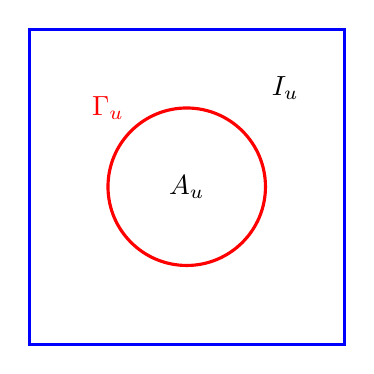
\begin{tikzpicture}
					% Draw the square with blue line and label it
					\draw[line width=0.4mm, blue] (0,0) rectangle (4,4);
			
					% Draw the circle with red line and label it
					\draw[line width=0.4mm, red] (2,2) circle (1cm);
					\node at (2,2) {{$A_u$}};
					\node at (1,3) {\textcolor{red}{$\Gamma_u$}};
			
					% Label the region between the circle and the square
					\node at (3.25,3.25) {$I_u$};
				\end{tikzpicture}
			\end{figure}
		\end{column}
	\end{columns}
\end{frame}

\begin{frame}
	\frametitle{Variational Inequalities: Equivalent Formulations}
	\begin{theo}[FTVI; Kinderlehrer \& Stampacchia 2000]
	  Fix $g, f \in C^\infty(\Omega)$ with $g_D \in C(\overline{\Omega})$, $\psi \in C(\overline{\Omega})$, $g_D \leq \psi$ and 
	  \begin{equation*}
		K_\psi = \{v \in H^1_{g_D}(\Omega)| v \geq \psi\}
	  \end{equation*}
	  
	  Then the following are equivalent:
	  \begin{enumerate}
		\item[(a)] $u$ is a solution to the energy minimization formulation, 
		\begin{align*}
		  \underset{u \in K_\psi}{\text{ minimize: }}  &I(u) = \int_\Omega \frac{1}{2} \abs{\nabla u}^2 - fu 
		\end{align*}
		\item[(b)] $u$ is a solution to the variational inequality formulation,
		\begin{equation*}
		  \int_\Omega \nabla u \cdot \nabla(v - u) \geq \int_\Omega f(v - u), \quad \text{ for all } v \in K_\psi.
		\end{equation*} 
	  \end{enumerate}
	\end{theo}
  \end{frame}


  \begin{frame}
	\frametitle{Variational Inequalities: Complimentarity Problem}
	\begin{theo}[FTVI]
  If $u \in C(\overline{\Omega}) \cap C^2(\Omega)$, then (a) or (b) implies:
  \begin{enumerate}

		\item[(c)] $u$ is a solution to the complementarity problem (CP) formulation, for which the following hold over $\Omega$ a.e.

		  \begin{align*}
			-\nabla^2 u - f &\geq 0 \\
			u - \psi &\geq 0 \\
			(-\nabla^2u - f)(u - \psi) &= 0 
		  \end{align*}

	\end{enumerate}
\end{theo}
%\begin{enumerate}[a]
%	\item Good for physical understanding but not as general. 
%	\item A more general weak form. 
%	\item Strong form which is nice for finite dim. algorithms. 
% \end{enumerate}
\end{frame}



\begin{frame}
	\frametitle{Variational Inequalities: Ball Obstacle Reference}
	\begin{itemize}
	  \item Exact solutions in 1d and 2d for ball obstacles. (Bueler 2021)
	\end{itemize}
  
	\begin{columns}[t] % Use [t] for top alignment
	  \column{0.5\textwidth}
	  \begin{figure}
		\centering
		\begin{tikzpicture}
		  \begin{axis}[
			width=0.9\textwidth, % Adjust the width of the plot
			height=0.7\textwidth, % Adjust the height of the plot
			axis lines=left,
			xlabel=x,
			ylabel={y},
			ylabel style={rotate=-90}, 
			xmin=0, xmax=2,
			ymin=0, ymax=1.5,
			no markers,
			samples=100,
			]
			\addplot [domain=0.697965148223374:2, samples=100, smooth] {-0.680259411891719*ln(x) + 0.471519893402112};
			\addplot [domain=0:0.697965148223374, samples=100, smooth] {sqrt(1 - x^2)};
			\addplot [blue, domain=0:.9, samples=100, smooth] {sqrt(1 - x^2)}; 
			\addplot [red, domain=0:1.5] ({0.697965148223374},x); 
			\node at (axis cs:1,1) [red] {a}; 
			\node at (axis cs:.35,1.25) [black] {$A_u$};
			\node at (axis cs:1.5, .5) [black] {$I_u$};
			\node at (axis cs:1,.25) [blue] {$\psi(r)$};
		  \end{axis}
		\end{tikzpicture}
	  \end{figure}
  
	  \column{0.5\textwidth}
	  \begin{figure}
		\centering
		\includegraphics[width=\textwidth]{Figures/Solution.png} % Replace with your image path
	  \end{figure}
	\end{columns}
  \end{frame}


\begin{frame}\frametitle{Variational Inequalities: Active Set Newton's Method}
	\begin{itemize}
		\item This problem is nonlinear so ...
		\begin{itemize}
			\item VI-adapted Newton Solver with Reduced Space Line Search.
			\begin{itemize}
				\item \texttt{vinewtonrsls} in PETSc
				\item (Benson \& Munson 2006)
			\end{itemize} 
			\item Solves finite nonlinear complementarity problems(NCP) with the form, 
			\begin{equation*}
				F(w) \geq 0, \quad w \geq 0, \quad F(w)w = 0.
 			\end{equation*}
		\end{itemize}
		\item To write the obstacle problem as an NCP:
		\begin{equation*}
			\underset{\text{Continuum CP}}{\begin{aligned}
			  -\nabla^2u - f &\geq 0\\
			  u - \psi &\geq 0\\
			  (-\nabla^2u - f)(u - \psi) &= 0
			\end{aligned}}
			\quad
			\underset{\shortstack{\scriptsize \text{Discretize}\\ \scriptsize \text{\&}\\ \scriptsize \text{Substitute}}}{\implies}
			\quad
			\underset{\text{Finite Dimensional NCP}}{\begin{aligned}
			  F(w) &\geq 0\\
			  w &\geq 0\\
			  F(w)w &= 0 
			\end{aligned}}
		  \end{equation*}
	\end{itemize}
	
\end{frame}

% \begin{frame}
% 	\begin{algorithm}[H]
% 	\begin{algorithmic}[1]
% 	\REQUIRE $w^k$.
% 	\STATE Define $A(w^k)$ "active (for now)" and $I(w^k)$ "undecided" vertex sets.
% 	\STATE Compute reduced space Newton step on $I(w^k)$.
% 	\begin{equation*}
% 		J(w^k)_{I^k, I^k}d_{I^k} = -F(w^k)_{I^k}.
% 	  \end{equation*}
% 	\STATE Define $d = [0, d_{I_k}]$.
% 	\STATE Apply projected line-search $\pi(w^k + \beta d)$ for admissibility in $K = \{w \in \RR^n: w \geq 0\}$.
% 	\STATE Update $w^{k+1} = \pi(w^k + \beta d)$.
% 	\end{algorithmic}
% 	\caption{vinewtonrsls: VI-adapted Newton's Method}
% 	\label{alg:seq}
% 	\end{algorithm}
% 	\end{frame}


% 	\begin{frame}[fragile]
% 	\frametitle{Finite Element Method: 2d Ball Obstacle Problem}
	
% 	\begin{lstlisting}[language=Python, basicstyle=\ttfamily\tiny]
% ... 
% (x, y) = SpatialCoordinate(mesh)
% r = sqrt(x * x + y * y)
% r0 = 0.9
% psi0 = np.sqrt(1.0 - r0 * r0)
% dpsi0 = - r0 / psi0
% psi_ufl = conditional(le(r, r0), sqrt(1.0 - r * r), psi0 + dpsi0 * (r - r0))
% lb = Function(V).interpolate(psi_ufl)

% afree = 0.697965148223374
% A = 0.680259411891719
% B = 0.471519893402112
% uexact_ufl = conditional(le(r, afree), psi_ufl, - A * ln(r) + B)
% uexact = Function(V).interpolate(uexact_ufl)

% bdry_ids = (1, 2, 3, 4) 
% bcs = DirichletBC(V, uexact, bdry_ids)

% F = inner(grad(u), grad(v)) * dx
% sp = {"snes_type": "vinewtonrsls",
% 	  # Newton step equations are solved by LU
% 	  "ksp_type": "preonly",
% 	  "pc_type": "lu",
% 	  "pc_factor_mat_solver_type": "mumps"}

% problem = NonlinearVariationalProblem(F, u, bcs)
% solver = NonlinearVariationalSolver(problem, solver_parameters=sp)
% solver.solve(bounds=(lb, ub))  	
% 	\end{lstlisting}

% 	\url{https://www.firedrakeproject.org/}
%   \end{frame}


  \begin{frame}
	\frametitle{Various "Conforming" Admissibility}
	\begin{definition}[FE VI Solution]
		Let $\cK_h = \{v_h \in H^1_{g_D}(\Omega)| v_h \geq \psi_h\}$ be the feasible set.
		\vfill
		Our FE method seeks $u_h \in \cK_h$ which satisfies
				\begin{equation*}
		  \int_\Omega \nabla u_h \cdot \nabla(v_h - u_h) \geq \int_\Omega f(v_h - u_h), \quad \text{ for all } v_h \in \cK_h.
		\end{equation*} 
	\end{definition}
	There are levels of conformity,
	\begin{itemize}
		\item[1] $\cK_h \not\subset \cK$ (e.g. $\psi_h$ is a P1 interpolant)
		\vfill
		\item[2] $\cK_h \subset \cK$ (e.g. $\psi_h$ is a P1 interpolant + monotone injection operator (Bueler \& Farrell 2024))
		\vfill
		\item[3] $\cK_h = \cK \cap \cX_h$ ($\psi$ exactly representable in FE space)
	\end{itemize}
  \end{frame}

  \begin{frame}
	\begin{definition}[Preferred Approximation]
		Let $u_h$ be the FE solution to the VI problem with computed active set $A^h_u$. The preferred approximation $\tilde{u}_h$ as the measurable function, 
		\begin{equation} 
\tilde u_h(x) = \begin{cases} \psi(x), & x\in A_u^h \\ u_h(x), & \text{otherwise.} \end{cases}
\end{equation}
	\end{definition}
	The error decomposes into active and inactive set contributions,
	\begin{equation*}
\|u-\tilde u_h\|_2^2 = \int_{ A_u\cap A_u^h} |\psi - \psi|^2 + \int_{A_u\setminus A_u^h} |\psi - u_h|^2 + \int_{A_u^h\setminus A_u} |u - \psi|^2 + \int_{I_u\cap I_u^h} |u-u_h|^2. 
\end{equation*}
\begin{itemize}
	\item Accurate free boundary approximation minimizes the middle two terms.
	\item PDE error estimators only control the last term.
\end{itemize}

\end{frame}




\begin{frame}
	\frametitle{Active Set Residual Measure}
\begin{definition} Suppose $u\in \cK$ solves the continuum VI.  Then $F(u)-\ell=d\mu_u$ is a positive Radon measure supported in $A_u$.  Thus for $w\in\cX$ we have
\begin{equation}
(F(u)-\ell)[w] = \int_{A_u} w\, d\mu_u. \label{eq:measure}
\end{equation}
\end{definition}
\end{frame}


\begin{frame}
	\frametitle{Why Regular PDE Error Estimators Won't Work}
	\begin{itemize}
		\item For a VI solution $u$ the active set residual is very different from a PDE residual.
	\end{itemize}
	\begin{figure}
		
		\begin{columns}
			\begin{column}{0.48\textwidth}
				\includegraphics[width=\textwidth]{OnEntireDomain.png}
			\end{column}
			\begin{column}{0.48\textwidth}
				\includegraphics[width=\textwidth]{OnInactiveSet.png}
			\end{column}
		\end{columns}
		\caption{AMR with BR estimator on entire domain (left) and inactive set (right).}
	\end{figure}
\end{frame}



\begin{frame}
\frametitle{Variational Inequalities: A Priori Error}


\begin{corollary}[2.5 (Fochesatto \& Bueler)] Suppose $u\in\cK$ solves the continuum VI and $u_h\in\cK_h$ solves the FE VI and $\psi \in C^1(\Omega)$.
\begin{align*}
\|u-u_h\|^2 \lesssim &\inf_{v\in\cK} \int_{A_u} (v-u_h)\,d\mu_u + \inf_{v_h\in\cK_h} \int_{A_u} (v_h-\psi)\,d\mu_u \\
&\, + \inf_{v_h\in\cK_h} \left(\int_{A_u} |\grad v_h - \grad \psi|^2\,dx + \int_{I_u} |\grad v_h - \grad u|^2\,dx\right)
\end{align*}
\end{corollary}

As long as $\Gamma_h \approx \Gamma$ the first three terms don't require mesh refinement to improve the FE solution. 
\end{frame}



%	\begin{frame}\frametitle{Variational Inequalities: Active Set Newton's Method}
%		\begin{algorithm}[H]
%			\caption{VINEWTONRSLS}
%			\begin{algorithmic}[1]
%			  \Require $w^k$.
%			  \State Define $A(w^k)$ "certainly active" and $I(w^k)$ "undecided" vertex sets.
%			  \State Compute $d$ via a reduced space Newton step on $I(w^k)$.
%			  \State Perform a line search along $\pi(w^k + \beta d)$ to stay inside $K = \{w \in \RR^n: w \geq 0\}$.
%			  \State Update $w^{k+1} = \pi(w^k + \beta d)$.
%			\end{algorithmic}
%			\end{algorithm}
%		\end{frame}
		
	







%\begin{frame}
%	\frametitle{Variational Inequalities: Convergence Experiment}
%
%	To demonstrate how convergence differs between VI and PDE problems, we solved the following problems:
%
%		\begin{columns}[t] % Align columns at the top
%			\column{0.45\textwidth}
%			% Add content for the first column here
%			\begin{block}{NCP Problem}
%				\begin{align*}
%					\Omega &= [-1, 1]\\
%					u(-1) &= u(1) = 0\\\\
%					u'' &\geq 0 \\
%					u - (1/2 - x^2) &\geq 0 \\
%					(u'')(u - (1/2 - x^2)) &= 0 
%				  \end{align*}
%			\end{block}
%		
%			\column{0.45\textwidth}
%			% Add content for the second column here
%			\begin{block}{PDE Problem}
%				\begin{align*}
%					\Omega &= [-1, 1]\\
%					u(-1) &= u(1) = 0\\\\
%					u'' &= 1
%				  \end{align*}
%
%			\end{block}
%		
%		  \end{columns}
%
%
%\end{frame}


\begin{frame}
\frametitle{QoI: Free Boundary Location?} % Fixed typo
\begin{itemize}
\item Simulation goal is locating the free boundary.
\vfill
\item Active Set dominated problems.
\vfill
\item Apply correct type of AMR on Inactive Set. (Possible DWR and admissable P-adaptivity etc.)
\vfill
\item Many methods (FASCD and VINEWTON) benefit from Free Boundary aware AMR.
% \begin{itemize}
% \item Modify multigrid (FASCD)
% \begin{itemize}
% \item Monotone restriction and prolongation require low order basis
% \item Mildly mesh dependent convergence
% \item Fancy Implementation
% \end{itemize}
% \item Modify basis functions (Bernstien Polynomials)
% \begin{itemize}
% \item Also mildly mesh dependent convergence
% \item Fancy implementation
% \end{itemize}
% \item Proximal Galerkin (LVPP)
% \begin{itemize}
% \item Would probably also benefit from Free Boundary aware AMR.
% \end{itemize}
% \end{itemize}
\end{itemize} % Corrected nesting closure
\end{frame}










  \section{Adaptive Mesh Refinement}
  \tableofcontents[currentsection]


  \begin{frame}
	\frametitle{Adaptive Mesh Refinement: Tagging Methods}
	\begin{itemize}
	  \item Refinement Loop:
		\begin{enumerate}
		  \item \textbf{Solve}: Compute the solution on the current mesh.
		  \item \textbf{Estimate}: Estimate error for each element.
		  \item \textbf{Tag}: Tag elements for refinement based on estimate.
		  \item \textbf{Refine}: Refine mesh while maintaining minimum angle criteria.
		\end{enumerate}
		\vfill
		Implementation: \texttt{github.com/StefanoFochesatto/viamr}
		\item Firedrake will address the Solve step.
		\item PETSc/Netgen (Zerbinati et al. 2024) integration will address the Refine step.
	\end{itemize}

  \end{frame}


%  \begin{frame}
%	\frametitle{Adaptive Mesh Refinement: Mesh Refinement}
%	Considerations
%	\begin{itemize}
%	  \item Minimum angle condition. 
%	  \item Hanging nodes. 
%	\end{itemize}
%	\begin{figure}
%		\centering
%		\definecolor{ffqqqq}{rgb}{1.,0.,0.}
%		\definecolor{uuuuuu}{rgb}{0.26666666666666666,0.26666666666666666,0.26666666666666666}
%		\definecolor{xdxdff}{rgb}{0.49019607843137253,0.49019607843137253,1.}
%	  
%		\begin{tikzpicture}[line cap=round, line join=round, >=triangle 45, scale=.6, x=1.5cm, y=1.5cm]
%		  \clip(2.5, -2.) rectangle (7.5, 2.);
%		  \draw [line width=1.pt] (3., 0.) -- (5.013325073747922, 1.544475570087121);
%		  \draw [line width=1.pt] (5.013325073747922, 1.544475570087121) -- (5.013325073747922, -1.535428203717027);
%		  \draw [line width=1.pt] (5.013325073747922, -1.535428203717027) -- (3., 0.);
%		  \draw [line width=1.pt] (5.013325073747922, -1.535428203717027) -- (7., 0.);
%		  \draw [line width=1.pt] (5.013325073747922, 1.544475570087121) -- (7., 0.);
%		  
%		  \draw [line width=1.pt, color=green] (4.006662536873961, 0.7722377850435606) -- (4.006662536873961, -0.7677141018585135);
%		  \draw [line width=1.pt, color=green] (5.013325073747922, 0.004523683185047034) -- (4.006662536873961, -0.7677141018585135);
%		  \draw [line width=1.pt, color=green] (4.006662536873961, 0.7722377850435606) -- (5.013325073747922, 0.004523683185047034);
%		  
%		  \begin{scriptsize}
%			\draw [fill=xdxdff] (3., 0.) circle (2.5pt);
%			\draw [fill=xdxdff] (7., 0.) circle (2.5pt);
%			\draw [fill=xdxdff] (5.013325073747922, 1.544475570087121) circle (2.5pt);
%			\draw [fill=xdxdff] (5.013325073747922, -1.535428203717027) circle (2.5pt);
%			\draw [fill=uuuuuu] (4.006662536873961, 0.7722377850435606) circle (3.5pt); % Larger black point
%			\draw [fill=ffqqqq] (5.013325073747922, 0.004523683185047034) circle (3.5pt); % Larger red point
%			\draw [fill=uuuuuu] (4.006662536873961, -0.7677141018585135) circle (3.5pt); % Larger black point
%		  \end{scriptsize}
%		\end{tikzpicture}
%		\caption*{Refinement (green) and hanging node (red).}
%	  \end{figure}
%  \end{frame}
%
%
%
%  \begin{frame}
%	\frametitle{Transition Cells: Handled by Netgen}
%	\myfigure{.85}{Figures/TransitionCells.png}{Example of Transition Cell.}
%	\begin{itemize}
%		\item Refinement region is expanded. 
%		\item Netgen's \texttt{.refine\_marked\_elements()} uses transition cells. 
%	\end{itemize}
%  \end{frame}
%
%  \begin{frame}
%	\frametitle{Interpolation into DG0}
%	\begin{columns}
%    
%		\begin{column}{0.45\textwidth}
%			\begin{itemize}
%				\item A DG0 finite element space has basis functions $\phi_i$, constant over each element.
%			\end{itemize}
%		\end{column}
%	
%		\begin{column}{0.50\textwidth}
%			\begin{figure}
%				\centering
%				\includegraphics[width=.8\textwidth]{Figures/DG0Basis.png}
%				\caption*{DG0 Basis Function $\phi_i$}
%			\end{figure} % Make sure caption works by enabling caption package if necessary
%		\end{column}
%	
%	\end{columns}
%	
%		\vfill
%		\begin{definition}[Interpolation into DG0]
%			$interpolate(u) = \sum_{i = 1}^n v_i \phi_i$ where
%			\begin{equation*}
%				v_i = \frac{1}{area(\triangle_i)}\int_{\triangle_i} u \, dx.
%			\end{equation*} 
%		\end{definition}
%  \end{frame}
%
\section{Two New Methods: VCD and UDO}
\tableofcontents[currentsection]

\begin{frame}
	\begin{itemize}
		\item The goal is to tag elements near the free boundary for refinement.
	\end{itemize}
		\begin{enumerate}
			\item Variable Coefficient Diffusion (VCD). 
			\item Unstructured Dilation Operator (UDO).
			\item Averaged-metric Method (AVM). 
		\end{enumerate}
\end{frame}


\begin{frame}
	\frametitle{Variable Coefficient Diffusion (VCD)}
	\begin{figure}[H]
		\centering
		\includegraphics[width=.65\textwidth]{Figures/VCESIllustration.png}
		\caption*{Illustration of VCD.}
		
	\end{figure}
\end{frame}



  \begin{frame}
	\begin{algorithm}[H]
	\caption{VCD Element Tagging for VIs}
	\begin{algorithmic}[1]
		\REQUIRE mesh $\cT_h$, solution $u_h \in \cK_h$, obstacle $\psi_h \in \cX_h$, tolerance $\text{tol} > 0$, and threshold interval $0 < \alpha < \beta < 1$.
		\STATE Compute nodal active set indicator $\nu_h \in \cX_h$ for $u_h$.
		\STATE For $h_K$ the element diameter, let $D=0.5 h_K^2 \in \DG_0(\cT_h)$.
		\STATE Approximately solve for $s_h\in\cX_h$, with natural boundary conditions:
		\begin{equation}
            s_h - \Div(D \grad s_h) = \nu_h
		\end{equation}
		\RETURN marking $1_h \in \DG_0(\cT_h)$ of all elements such that $s_h(x_k) \in (\alpha,\beta)$.
	\end{algorithmic}
	\end{algorithm}
	\begin{itemize}
		\item $D$ is set so diffusion range $\propto$ element diameter
		\item Solve Eq.(3) with 4 iterations of Incomplete Cholesky-preconditioned CG ($O(V)$ complexity).
	\end{itemize}
	\end{frame}



%   \begin{frame}
% 	\frametitle{DMPlex (component of PETSc)}
% 	\begin{itemize}
% 		\item Mesh entities (vertices, edges, faces, cells) and a covering relation are represented by directed acyclic graph (DAG)
% 	\end{itemize}
% 	\begin{figure}[H]
% 		\centering
% 		\includegraphics[width=.9\textwidth]{Figures/DMPlexExample.png}
% 		\caption*{DMPlex representation of a mesh.}
% 	\end{figure}
% \end{frame}

\begin{frame}
	\frametitle{Unstructured Dilation Operator}	
	\begin{definition}[Neighborhood Depth Parameter]
		Let $T$ be a triangulation of $\Omega$. We define the function $N(\triangle)$ as follows:
		\begin{equation*}
			N(\triangle) = \{\triangle_i \in T: \triangle \text{ shares at least 1 vertex with } \triangle_i\}.
		\end{equation*}
		We define the $n$ composition of $N$ as follows: 
		\begin{equation*}
			N^n(\triangle) = \underbrace{N(...N(\triangle))}_{n \text{ times}}.
		\end{equation*}
		We will refer to $n$ as the neighborhood depth parameter.
	\end{definition}
\end{frame}





\begin{frame}
	\frametitle{Unstructured Dilation Operator}
	\begin{figure}
		\centering
		\includegraphics[width=.6\textwidth]{Figures/UDOIllustration/000.png}
	\end{figure}
\end{frame}


% \begin{frame}
% 	\frametitle{Unstructured Dilation Operator: Illustration}
% 	\begin{figure}
% 		\centering
% 		\includegraphics[width=.8\textwidth]{Figures/UDOIllustration/001.png}
% 	\end{figure}
% \end{frame}


\begin{frame}
	\frametitle{Unstructured Dilation Operator}
	\begin{figure}
		\centering
		\includegraphics[width=.6\textwidth]{Figures/UDOIllustration/002.png}
	\end{figure}
\end{frame}


\begin{frame}
	\frametitle{Unstructured Dilation Operator}
	\begin{figure}
		\centering
		\includegraphics[width=.6\textwidth]{Figures/UDOIllustration/003.png}
	\end{figure}
\end{frame}


  \begin{frame}
	\begin{algorithm}[H]
		\caption{UDO Element Tagging for VIs}
		\begin{algorithmic}[1]
		\REQUIRE mesh $\cT_h$, solution $u_h \in \cK_h$, obstacle $\psi_h \in \cX_h$, tolerance $\text{tol} > 0$, and expansion parameter $n\ge 1$.
		\STATE Compute nodal active set indicator $\nu_h \in \cX_h$ for $u_h$.
		\STATE Find initial element index set $S_0$: \,$k\in S_0$ if $\nu_h(x_k) \in (0,1)$.		
		\STATE Use DMPlex to facilitate construction of $S_n = N^n(S_0)$.
		\RETURN marking $1_h \in \DG_0(\cT_h)$ of all elements with indices in $S_n$.
		\end{algorithmic}
	  \end{algorithm}
	% Algorithm
  \end{frame}



  \begin{frame}
	\begin{algorithm}[H]
	\caption{Averaged-metric (AVM) mesh adaptation}
	\begin{algorithmic}[1]
		\REQUIRE mesh $\cT_h$, solution $u_h \in \cK_h$, obstacle $\psi_h \in \cX_h$, target complexity $N$, element diameter bounds $0<\hmin<\hmax$, and averaging weight $0\le \gamma \le 1$
		\STATE Compute $s_h \in \cX_h$ from VCD, using $u_h$ and $\psi_h$.
		\STATE Compute normalized isotropic free-boundary metric: \\
		$M_1(x)=c_1 |\grad s_h(x)| I_{d\times d}$.
		\STATE Compute normalized anisotropic metric from Hessian: \\
		$M_2(x)=c_2 |H u_h(x)|$.
		\STATE Average the metrics: $M(x) = \gamma M_1(x) + (1-\gamma) M_2(x)$. \\
		\RETURN new mesh $\tilde \cT_h$ which is unit with respect to $M(x)$.
    \end{algorithmic}
\end{algorithm}
\end{frame}





\section{Results}
\tableofcontents[currentsection]



\begin{frame}
	\frametitle{Mesh Refinement Examples: 7 iterations of VCD}
		\begin{columns} % Align columns at the top
			\column{0.5\textwidth}
			\begin{figure}[H]
				\centering
				\includegraphics[width=.8\textwidth]{Figures/7step45to65smoothing.png}
				\caption*{$(\alpha, \beta) =  (.45, .65)$.}
				\label{fig:image1}
			\end{figure}
				
			\column{0.5\textwidth}
			\begin{figure}[H]
				\centering 
				\includegraphics[width=.8\textwidth]{Figures/7step91smoothing.png}
				\caption*{$(\alpha, \beta) = (.1, .9)$.}
				\label{fig:image2}
			\end{figure}
		  \end{columns}
  \end{frame}


  \begin{frame}
	\frametitle{Mesh Refinement Examples: 7 iterations of UDO}
		\begin{columns}[t] % Align columns at the top
			\column{0.5\textwidth}
			\begin{figure}[H]
				\centering
				\includegraphics[width=.8\textwidth]{Figures/7step1neighbor.png}
				\caption*{$n = 1$}
				\label{fig:image1}
			\end{figure}
		  \column{0.5\textwidth}
		  \begin{figure}
			\centering
			\includegraphics[width=.8\textwidth]{Figures/7step5neighbor.png}
			\caption*{$n = 5$}
		\end{figure}
		  \label{fig:image2}
		\end{columns}
  \end{frame}



%   \begin{frame}
% 	\frametitle{Preliminary Results: Spiral Obstacle}
% 		\begin{columns}[t] % Align columns at the top
% 			\column{0.5\textwidth}
% 			\begin{figure}[H]
% 				\centering
% 				\includegraphics[width=\textwidth]{Figures/7step91smoothingspiral.png}
% 				\caption*{VCD: $(\alpha, \beta) = (.1, .9)$}
% 				\label{fig:image1}
% 			\end{figure}
% 		  \column{0.5\textwidth}
% 		  \begin{figure}
% 			\centering
% 			\includegraphics[width=\textwidth]{Figures/7step1neighborspiral.png}
% 			\caption*{UDO: $n = 1$}
% 		\end{figure}
% 		  \label{fig:image2}
% 		\end{columns}
%   \end{frame}

\begin{frame}
	\begin{figure}[ht]
\centering
\includegraphics[width = .4\textwidth]{../../paper/static/spiralmesh.png}
\caption{A spiral obstacle example with $2\times 10^5$ elements, 7x UDO$+$BR with initial mesh of 200 elements.  Element diameter (resolution) is $h\approx 10^{-3}$ along the free boundary.}
\label{fig:spiralmesh}
\end{figure}
\end{frame}

  \begin{frame}
	\frametitle{Quality Metric for Free Boundary Approximation}
	\begin{definition}[Jaccard distance]
		The Jaccard distance between measurable sets $S, T \subset \Omega$ is
		\begin{equation*}
			d(S, T) = 1 - \frac{\abs{S \cap T}}{\abs{S \cup T}}
		  \end{equation*}
		  where $\abs{\cdot}$ is the Lebesgue measure, with $d(S, T) = 0$ by definition if $\abs{S \cup T} = 0$.
	\end{definition}
	\begin{itemize}
		\item \texttt{viamr.jaccard()} parallel implementation works for DG0 and UFL indicator functions. 
	\end{itemize}
  \end{frame}



\begin{frame}
	
\begin{figure}[ht]
\includegraphics[width=0.60\textwidth]{../../paper/genfigs/convball_UDO+BR.png}
\caption{$L^2$ norm errors for the UDO$+$BR versus uniform on mostly active set problem with preferred solution $\tilde{u_h}$ }
\end{figure}
\end{frame}



\begin{frame}
	\begin{figure}[ht]
\centering
\includegraphics[width=0.60\textwidth]{../../paper/genfigs/jaccball.png}
\caption{Active set Jaccard distances $d(A_u^h,A_u)$.}
\end{figure}
\end{frame}











\begin{frame}
    \frametitle{More Mesh Refinement Examples}
    \begin{figure}
        \centering
        \includegraphics[width=0.40\textwidth]{../../paper/static/blistersmesh.png}
        \hfill % Puts flexible space between the images
        \includegraphics[width=0.40\textwidth]{../../paper/static/blisterszoomed.png}
        \caption{A mesh for active set dominated problem of $4.7\times 10^5$ elements, with resolution $h\approx 10^{-3}$ along the free boundary, from four levels of the VCD$+$BR approach, starting from a uniform mesh of 1800 elements.}
        \label{fig:blistersmesh}
    \end{figure}
\end{frame}

\begin{frame}
	\begin{figure}[ht]
\centering
\includegraphics[height=62mm]{../../paper/static/lshaped.png}
\caption{A refined mesh from three iterations of AVM Algorithm an L-Shaped domain problem, showing a well-resolved free boundary and refinement in the interior corner.}
\end{figure}
\end{frame}




\begin{frame}
    \frametitle{Application: Determining Glaciated Land Areas}
	\begin{block}{Goal}
    Solve for the area of land covered by ice, also known as the \textbf{glaciated area}.
    \end{block}

    
    The model uses the \textbf{shallow ice approximation} with a standard shear-thinning flow law for ice. This results in a VI based on a "tilted" variation of the $p$-Laplacian operator.
    
    
\end{frame}

\begin{frame}
	    \frametitle{Application: Determining Glaciated Land Areas}
		    \begin{alertblock}{Variational Inequality Formulation}
    Find $u \in \mathcal{K}$ such that for all $v \in \mathcal{K}$:
    $$
    \int_\Omega \Gamma |\nabla u + \mathbf{\beta}(u)|^2 (\nabla u + \mathbf{\beta}(u)) \cdot \nabla (v-u) - \tilde a(u) (v-u)\,dx \ge 0
    $$
    \end{alertblock}

	    \begin{block}{Function Spaces \& Physical Variables}
    We solve for a transformed ice thickness $u$:
\begin{columns}[T] % The [T] option aligns the columns at the top
    
    % --- LEFT COLUMN ---
    \begin{column}{0.5\textwidth}
        \begin{itemize}
            \item \textbf{Physical ice thickness}: $H = u^{3/8}$
            \item \textbf{Ice surface elevation}: $s = u^{3/8} + b$
            \item \textbf{Bedrock elevation}: $b(x,y)$
            \item \textbf{Surface mass-balance}: $a(x,y,s)$
        \end{itemize}
    \end{column}
    
    % --- RIGHT COLUMN ---
    \begin{column}{0.5\textwidth}
        \begin{itemize}
            \item \textbf{Ice softness}: $\Gamma > 0$
            \item \textbf{Tilt term}: $\mathbf{\beta}(u)=\frac{8}{3} u^{5/8} \nabla b$
            \item $\tilde a(u)=a(x,y,s)$
            \item $u \in \cK = \{u \in W^{1,4}(\Omega)\,:\,u\ge 0 \text{ and } u|_{\partial\Omega}=0\}$
        \end{itemize}
    \end{column}
    
\end{columns}
    \end{block}

	\begin{itemize}
		\item Generally $|\grad s| \to \infty$ at the glacier margin.
	\end{itemize}

\end{frame}




\begin{frame}
	    \frametitle{Application: Determining Glaciated Land Areas}
	Let $\Omega=(0,L)^2$ with $L=1800$ kilometers. With flat bed, elevation-independent source, and a known exact solution (Bueler 2016)

    \begin{block}{Simulation Setup}
        \begin{itemize}
            \item \textbf{Refinement Strategy:} 13 levels of adaptive mesh refinement (AMR).
            \item \textbf{Initial Mesh:} Uniform grid with element size $h_0 = 360$ km.
            \item \textbf{Final Resolution:} High resolution at the glacier margin, $h_{13} \approx 30$ m.
            \item \textbf{AMR Algorithms:} Both UDO+GR and VCD+GR methods were applied with similar results.
        \end{itemize}
    \end{block}
    
\end{frame}


\begin{frame}
        \begin{columns}[T]
        \begin{column}{0.5\textwidth}
     \begin{figure}
        \centering
        \includegraphics[width=\textwidth]{../../paper/genfigs/drmax.png}
        \caption*{Maximum radial error of the glacier margin.}
    \end{figure}
        \end{column}
        \begin{column}{0.5\textwidth}
            \begin{figure}
                \includegraphics[width=\textwidth]{../../paper/genfigs/herrinf.png}
                \caption*{Max error in the ice thickness $H$.}
            \end{figure}
        \end{column}
    \end{columns}
    
\end{frame}



\begin{frame}
	\frametitle{Conclusion}
	\begin{itemize}
		\item Stabilizing Active/Inactive Sets is important.
		\begin{itemize}
			\item Efficiency in computation on Active Set. 
			\item Correct type of PDE AMR on Inactive Set.
			\item Preferred Approximation uses data and is generally admissible. 
		\end{itemize}
		\vfill
		\item Parallel Firedrake implementation with examples in 2d and 3d \texttt{github.com/StefanoFochesatto/viamr}
		\item Associated Paper 
	\end{itemize}
\end{frame}


\begin{frame}
	\frametitle{Conclusion}
	\begin{itemize}
		\vfill
		\item Question?
		\vfill
	\end{itemize}
\end{frame}



\begin{frame}
	\frametitle{Acknowledgements}
	    \begin{itemize}
        \item Travel support provided by the University of Colorado Boulder 
	   \end{itemize}

\end{frame}


\begin{frame}[fragile] % Use [fragile] option because of the code
    \frametitle{Example: A Classical Obstacle Problem}
    \framesubtitle{Solving Ainsworth, Oden \& Lee (1993) with viamr + Firedrake}

    We solve a classical obstacle problem with a known exact solution ($\psi=0$). 
    The algorithm proceeds in three steps:
    
    % Use overlays to reveal points one by one
    \begin{itemize}
        \item<2-> Start with a uniform coarse mesh.
        \item<3-> Apply VCD marking to identify cells near the free boundary.
        \item<4-> Refine only the marked cells to generate the new mesh.
    \end{itemize}

    \vfill % Pushes the figures down a bit

    % Use a columns environment for a clean, multi-image layout
    \begin{columns}[T] % T option aligns the tops of the columns
        \begin{column}{0.32\textwidth}
            \centering
            \uncover<2->{Initial Mesh \\}
            \uncover<2->{\includegraphics[width=\columnwidth]{../../paper/static/aol-mesh.png}}
        \end{column}
        \begin{column}{0.32\textwidth}
            \centering
            \uncover<3->{Marked Cells (VCD) \\}
            \uncover<3->{\includegraphics[width=\columnwidth]{../../paper/static/aol-marked.png}}
        \end{column}
        \begin{column}{0.32\textwidth}
            \centering
            \uncover<4->{Refined Mesh \\}
            \uncover<4->{\includegraphics[width=\columnwidth]{../../paper/static/aol-refinedmesh.png}}
        \end{column}
    \end{columns}

    % Use a block to highlight the key takeaway
    \uncover<5->{
    \begin{alertblock}{Key Observation}
        The algorithm correctly avoids refining the inactive set, which is a necessary condition for convergence. The exact free boundary is shown in black.
    \end{alertblock}
    }

\end{frame}

\begin{frame}[fragile] % The [fragile] option is required for the minted environment
    % --- The Code Snippet ---
    % The 'fontsize=\footnotesize' option makes the code text smaller to fit.
    % You can also use \scriptsize or \tiny if you need it even smaller.
    \inputminted[linenos, frame=lines, fontsize=\scriptsize]{python}{../../examples/aol.py}

    \vfill % Adds flexible vertical space between the code and figures

\end{frame}





%   \begin{frame}
% 	\frametitle{VCD and UDO Parameter Sensitivity}
% 	\begin{figure}
% 		\centering
% 		\includegraphics[width=.85\textwidth]{Figures/ParameterExp.png}
% 	\end{figure}
%   \end{frame}
  


  
%   \begin{frame}
% 	\frametitle{Jaccard Index VCD}
% 	\begin{figure}
		
% 		\centering
% 		\includegraphics[width=\textwidth]{Figures/Convergence/elementsVIou.png}
% 	\end{figure}
% \end{frame} 

% \begin{frame}
%   \frametitle{Jaccard Index UDO}
%   \begin{figure}
	
% 	\centering
% 	  \includegraphics[width=\textwidth]{Figures/Convergence/elementsVIouUDO.png}
% 	\end{figure}
% \end{frame} 

% \begin{frame}
% 	\frametitle{Hausdorff Distance VCD}
% 	\begin{figure}
		
% 		\centering
% 		\includegraphics[width=\textwidth]{Figures/Convergence/elementsVhausdorff.png}
% 	\end{figure}
% \end{frame} 


% \begin{frame}
% 	\frametitle{Hausdorff Distance UDO}
% 	\begin{figure}
% 		\centering
% 		\includegraphics[width=\textwidth]{Figures/Convergence/elementsVhausdorffUDO.png}
% 	\end{figure}
% \end{frame} 

%   \begin{frame}
% 	\frametitle{Hybrid Refinement Strategy}
% 	\begin{itemize}
% 		\item Proposed methods don't reduce error over the inactive set. 
% 		\item A hybrid strategy combines uniform refinement and an AMR method. 
% 	\end{itemize}
%   \end{frame}

% \begin{frame}
%   \frametitle{$L_2$ VCD}
%   \begin{figure}

% 	  \centering
% 	  \includegraphics[width=\textwidth]{Figures/Convergence/elementsVl2.png}
%   \end{figure}
% \end{frame} 

% \begin{frame}
% 	\frametitle{$L_2$ UDO}
% 	\begin{figure}
% 		\centering
% 		\includegraphics[width=\textwidth]{Figures/Convergence/elementsVl2UDO.png}
% 	\end{figure}
%   \end{frame} 

% 	\begin{frame}
% 		Thanks for Listening!
% 	\end{frame}


% 	\begin{frame}\frametitle{Further Work}
% 		\begin{itemize}
% 			\item Investigate other VI problems.
% 			\item Further testing of VCD and UDO (parallel).
% 			\item FASCD + AMR.
% 			\item Implementation using PETSc. 
% 		\end{itemize}
% 		\end{frame}


% 	\begin{frame}\frametitle{References}
% 		\begin{itemize}
% 			\item Howard C. Elman, David J. Silvester, and Andrew J. Wathen. Finite Elements and Fast Itera-
% 			tive Solvers: with Applications in Incompressible Fluid Dynamics, 2005.
% 			\vfill
% 			\item Kinderlehrer, David, and Guido Stampacchia. An Introduction to 
% 			Variational Inequalities and Their Applications, 2000.
% 			\vfill

% 			\item Ed Bueler. PETSc for Partial Differential Equations: Numerical Solutions in C and Python, 2021. 
% 			\vfill
			
% 			\item Steven J. Benson and Todd S. Munson. Flexible Complementarity Solvers for Large-Scale Applications, 2002.
% 			\vfill
			
% 			\item Umberto Zerbinati, Patrick E Farrell, Joachim Schoberl, and Stefano Zampini. ngsPETSc: A Coupling Between NETGEN/NGSolve and PETSc, 2024.
% 		\end{itemize}
	
% 	\end{frame}

% 	\begin{frame}\frametitle{References Cont.}
% 	\begin{itemize}	
% 		\item Michael Lange, Matthew G. Knepley, and Gerard J. Gorman. Flexible, Scalable Mesh and Data Management using PETSc DMPlex, 2015.
% 		\vfill
% 	\end{itemize}
% 	\end{frame}


% 	\begin{frame}\frametitle{Appendix: PF Inequality }
% 		\begin{theo}[Poincaré-Friedrichs Inequality]
% 			If $\Omega$ is a bounded domain and $u \in H_{0}^1(\Omega)$ then there exists a $C_1 > 0$ depending only on $\Omega$ such that,
% 			\begin{equation*}
% 				\norm{\nabla u}{L_2} \leq  \norm{u}{H^1} \leq \sqrt{1 + C_1} \norm{\nabla u}{L_2}.
% 			   \end{equation*}
% 		  \end{theo}
% 	\end{frame}


% \begin{frame}\frametitle{Appendix: Parallel Considerations}

% 	\begin{figure}[H]
% 		\begin{columns}
% 			\begin{column}{0.5\textwidth}
% 				\centering
% 				\includegraphics[width=\textwidth]{Figures/DistributedAMR.png}
% 				\label{fig:image1}
% 			\end{column}
% 			\begin{column}{0.5\textwidth}
% 				\centering
% 				\includegraphics[width=\textwidth]{Figures/DistributedUnif.png}
% 				\label{fig:image2}
% 			\end{column}
% 		\end{columns}
% 	  \end{figure}
% 	\end{frame}
% 	\begin{frame}\frametitle{Appendix: Parallel Considerations}





%     \begin{table}
%         \centering
%         % Resize the table to fit the width of the slide
%         \resizebox{\textwidth}{!}{%
%             \begin{tabular}{|c|c|c|c|c|c|c|} \hline
%                 \multicolumn{7}{|c|}{Element Counts and Ratios Across Processes} \\ \hline
%                 \multirow{2}{*}{Process} & \multicolumn{3}{c|}{VCD} & \multicolumn{3}{c|}{Uniform} \\ \cline{2-7}
%                 & Active & Inactive & Inactive Ratio & Active & Inactive & Inactive Ratio \\ \hline
%                 1 & 173 & 327 & 0.171 & 51 & 219 & 0.081 \\ \hline
%                 2 & 188 & 390 & 0.204 & 59 & 656 & 0.242 \\ \hline
%                 3 & 170 & 373 & 0.195 & 44 & 570 & 0.210 \\ \hline
%                 4 & 162 & 415 & 0.217 & 86 & 608 & 0.225 \\ \hline
%                 5 & 131 & 407 & 0.213 & 60 & 655 & 0.242 \\ \hline
%             \end{tabular}
%         }
%         \caption*{Process element counts and ratios. VCD mesh has 2736 total elements, Uniform has 3008 total elements.}
%         \label{tab:element_counts}
%     \end{table}

% \end{frame}





  \begin{frame}\frametitle{Appendix: Active Set Newton's Method Formulas}
	\begin{itemize}
		\item Define new residual, 
		\begin{equation*}
			\hat{F}_i(w) = \begin{cases}
			  F_i(w) & \text{if } w_i > 0,\\
			  \min\{F_i(w), 0\} & \text{if } w_i = 0.
			\end{cases}
		  \end{equation*}

		  \item Define iterate's Active and Inactive sets,
		  \begin{align*}
			A(w^k) &= \{i \in \{1, ..., N\}| w_i^k = 0 \text{ and } F_i(w^k) > 0\},\\
			I(w^k) &= \{i \in \{1, ..., N\}| w_i^k > 0 \text{ or } F_i(w^k) \leq 0\}.
		  \end{align*}

		  \item Reduced Space Newton Step,
		  \begin{equation*}
			J(w^k)_{I^k, I^k}d_{I_k} = -F(w^k)_{I^k}.
		  \end{equation*}

		  \item Projected Line Search,
		  \begin{equation*}
			\pi(w)_i = \begin{cases}
			  w_i & \text{if } w_i > 0,\\
			  0 & \text{if } w_i \leq 0.
			\end{cases}
		  \end{equation*}
	\end{itemize}
\end{frame}


\begin{frame}
	\frametitle{Inactive Set A Posteriori Error: Gradient Recovery}
	\begin{definition}[Gradient Recovery]  Suppose $\cX_h=\CG_k$, $u_h\in\cX_h$. Define $\cY_h=\DG_{k-1}$ and note that $\grad u_h \in \cY_h^d$ (vector-valued). Let $G : \cX_h \to \cX_h^d$ be a linear operator called \emph{gradient recovery} (GR) so that $G(u_h)\approx \grad u_h$ in some sense.  Over an element $K \in\cT_h$, the corresponding error indicator $\eta_K\ge 0$ is then
	\begin{equation} \label{eq:gradrecoveryindicator}
	\eta_K^2 = \int_K \left|G(u_h) - \grad u_h\right|^2.
	\end{equation}
	
	\end{definition}
\end{frame}


\begin{frame}
	\frametitle{Inactive Set A Posteriori Error: Babu\v{s}ka--Rheinboldt}
	\begin{definition}[Babu\v{s}ka--Rheinboldt]Let $u \in H^1(\Omega)$ and $u_h\in\cX_h=\CG_1$ be analytic and FE solutions to the Poisson problem. Given the (strong) residual $r(u_h)=-\nabla^2 u_h - f$ of the Poisson equation, well-defined within each element $K$, the Babu\v{s}ka--Rheinboldt (BR) error estimator is


	\begin{equation} 
	\eta_K^2 = h_K^2 \int_K |r(u_h)|^2\,dx + \frac{h_K}{2}  \sum_{\gamma \in \partial K \setminus \partial \Omega} \int_{\gamma} \left\llbracket \grad u_h \cdot n \right\rrbracket^2\,dS,
	\end{equation}
	\end{definition}
\end{frame}







%%%%%%END%%%%%%%
\end{document}
